\batchmode
\documentclass[a4paper,10pt]{article}
\usepackage{graphicx}
\usepackage{fancyvrb}
\usepackage{color}
\usepackage{xcolor}
\usepackage{verbatim}
\usepackage{amssymb}
\usepackage{amsmath}
\usepackage{hyperref}
\usepackage{natbib}
\usepackage{caption}
\usepackage{subcaption}

\hypersetup{urlcolor=blue, colorlinks=true} 
\usepackage{float}

%used in SL section
\usepackage{mathptmx}
\usepackage{siunitx} %SI-einheiten
\usepackage{lmodern} %weitere mathematischen Symbole
\usepackage{placeins} %floatbarrier

\DeclareSIUnit\parsec{pc}
\DeclareSIUnit\lightyear{ly}
\DeclareSIUnit\year{yr}
\DeclareSIUnit\erg{erg}
\DeclareSIUnit\ster{ster}
\DeclareSIUnit\arcsec{arcsec}
\DeclareSIUnit\deg{deg}


\definecolor{gruen}{cmyk}{0.35,0.01,0.80,0.1}

\textheight=25.5cm
\textwidth=17.5cm
\voffset=0.cm
\hoffset=-0.0cm
\oddsidemargin -1cm
\evensidemargin -1cm
\topmargin -2cm
\baselineskip=0.900cm
\setlength{\parindent}{0in}

\graphicspath{{../figures/}}

\providecommand{\e}[1]{\ensuremath{\times 10^{#1}}}
\newcommand{\given}[2]{\ensuremath{P(#1|#2)}}
\newcommand{\x}[0]{\ensuremath{\vec{x}}}
\newcommand{\gauss}[3]{\ensuremath{\frac{1}{\sqrt{2\pi#2^2}}\text{exp}\left(- \frac{(#1-#3)^2}{2#2^2}\right)}}

% used in SL section
\newcommand{\todo}[2]{\textcolor{red}{\textbf{TODO (#1): #2}}}

\title{Static science FoM}
\author{}
\date{}


\begin{document}
\maketitle

One metric that we use for static science is the Dark Energy Task Force (DETF) Figure of Merit (FoM)
for dark energy, representing the strength of parameter constraints on $w_0$ and $w_a$.  We use
estimates of this quantity in years 1, 3, 6, and 10, without Stage III priors so as to emphasize the
constraining power of the LSST data alone.

{\bf Methodology:} Our forecasting approach follows that in the DESC SRD v1 in many respects:

\begin{itemize}
\item We consider weak lensing, large-scale structure, and galaxy clusters, including the covariance
between these probes.  More specifically, we include the tomographic shear-shear, galaxy-shear, and
galaxy-galaxy correlations (`3x2-point’ analysis), along with tomographic cluster number counts and
small-scale shear signals to constrain the halo mass function. We use the same length scales
(wavenumber $\ell$). 
\item We use the same parametric form for describing the WL sample $n_\text{eff}(z)$ and the LSS
sample $N(z)$, with parameters determined as a function of observing strategy.  The cluster sample
parameters are fixed to those in the DESC SRD and not permitted to vary as a function of observing
strategy, since the adopted cluster sample definition is at sufficiently low redshifts that all
strategies should enable cluster detection and characterization with roughly the same efficiency.
\item We use the same redshift range and tomographic binning as in the DESC SRD in Y1 and Y10 for
LSS, gradually increasing the number of bins for intermediate years (5, 7, 9, and 10 bins in Y1, Y3,
Y6, Y10).  The same WL tomographic bins were used in all years in the DESC SRD and in this work.
\end{itemize}

There are a few important differences from the DESC SRD.  First, we did not marginalize over
astrophysical systematic uncertainties: intrinsic alignments, galaxy bias, and the cluster
mass-observable relation.  In other words, the FoM we use here is purely a measurement of
statistical constraining power, and does not account for the fact that e.g. a deeper sample may
require a more complex parametric model for the aforementioned effects. The reason to simplify in
this way is that we found unstable behavior in the FoMs that was a result of our simplistic
astrophysical systematics parametrization and does not reflect the way a realistic analysis
methodology would evolve depending on the adopted strategy.  Thus, the FoMs themselves represent
unattainable constraining power; to avoid over-reliance on the actual numbers, we renormalize the
FoMs with respect to that of to the `kraken\_2026` strategy in Y1, to show {\em relative}
improvements in constraining power.

Second, we did not use the full non-Gaussian covariances, which reduce the constraining power from
small scales.  Gaussian covariances only were used.  The non-Gaussian terms should not have a strong
dependence on the survey depth and area and hence should have a small impact on our conclusions.

Third, we did the calculations for strategies as a function of depth (which changes the effective
LSS and WL number densities and redshift distribution) and area on a 3x3 grid in each year, and then
interpolated on that grid to produce a FoM emulator that gave results for all strategies.

\textbf{Ingredients:} We used the same sample definition as for the LSS metrics.  This gave a median
$i$-band $5\sigma$ depth across the survey, and a  total usable area.  The $5\sigma$ depth had to be
converted to a normalization and parameters of the redshift distributions for the LSS and WL
samples.  These calculations were done for a grid of values and then fit to the following parametric
forms.  In the equations below, $i_\text{depth}$ is the median depth and $i_\text{lim}$ is the
presumed $i$-band magnitude limit of the LSS sample, which is $i_\text{ilim} = i_\text{depth}-1$:
\begin{itemize}
\item LSS sample total number density on the sky $\bar{n}=37.8 \times 10^{0.359 (i_\text{lim} -
25)}$ arcmin$^-2$.
\item LSS $z_0 = 0.00627 (i_\text{lim}-25)^2 + 0.0188 (i_\text{lim}-25) + 0.272$, and LSS $\alpha =
0.0125*(i_\text{lim}-25)^2 - 0.025 (i_\text{lim}-25) + 0.909$.
\item WL effective source density is $n_\text{eff} = 4.33 (i_\text{depth}-25)^2 + 7.03 (i_\text{depth}-25) + 10.49$.
\item WL $z_0 = -0.0125 (i_\text{depth}-25) + 0.193$, and WL $\alpha = -0.069 (i_\text{depth}-25) +
0.876$.
\end{itemize}

These were estimated using the same process described in the DESC SRD for the OpSim v3 minion\_1016
strategy used there.

Caveats: \textbf{State limitations here.  Actually did not include clusters in the end, possibly TBD.}

\textbf{Future work:} In Eifler et al (in prep), we will extend and improve this formalize to
include the following features: (a) non-Gaussian covariances, (b) a fully-featured emulator based on
a Latin hypercube, (c) a better understanding of the impact of astrophysical uncertainties, and
produce an improved emulator for the static science FoM that will go into MAF.


\begin{figure}{\columnwidth}
\centering
 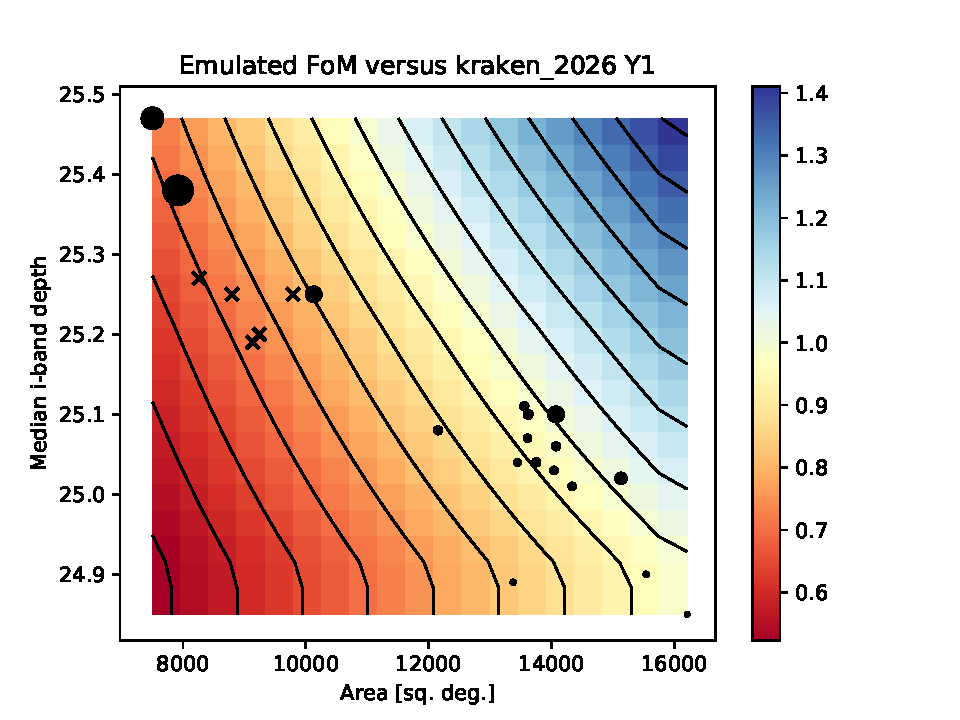
\includegraphics[width=0.45\columnwidth]{test_noprior_Y1_contour.pdf}
 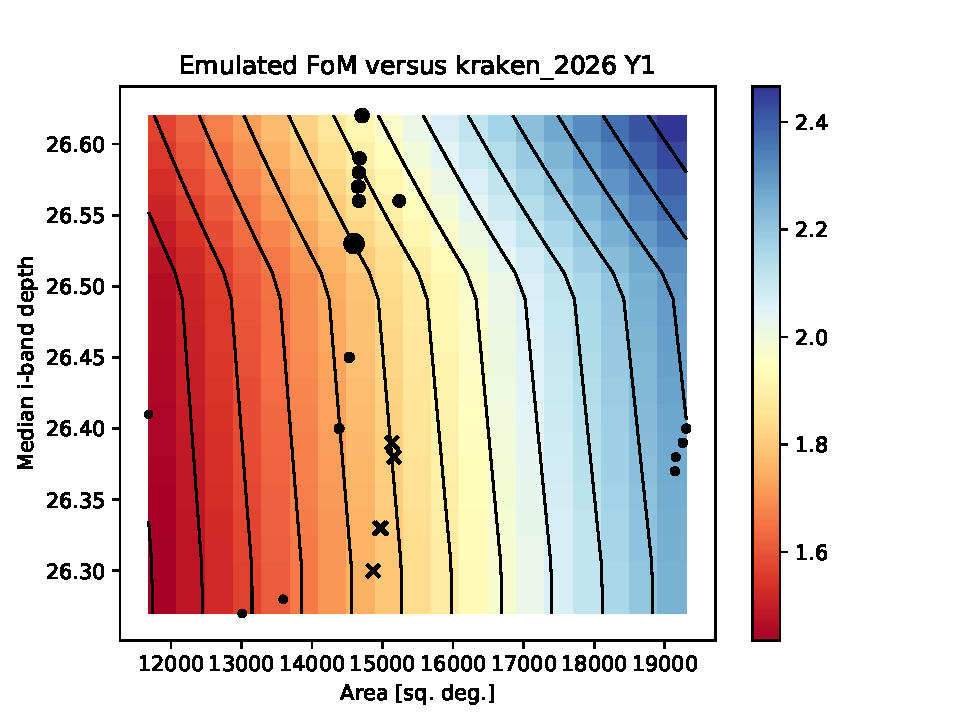
\includegraphics[width=0.45\columnwidth]{test_noprior_Y10_contour.pdf}
\caption{Y1 (left) and Y10 (right) FoM for the static science cases, normalized such that the
 `kraken\_2026' strategy gives a value of 1 in Y1.  Results are shown as a function of usable area
 for LSS versus median $i$-band depth, with the various strategies shown as crosses or points (if
 points, the point size indicates the value of the WL systematics metric, with larger points
 indicating better behavior with respect to systematics). As shown, the direction of contours in
 area vs.\ depth space differs for Y1 (which is shape noise dominated) and Y10 (which is cosmic
 variance dominated).\label{fig:static_fom}}
\end{figure}


\end{document}
